\documentclass[11pt,a4paper]{article}

\usepackage[a4paper,margin=0.75in,right=1in]{geometry}

\usepackage{amsmath,amssymb}
\usepackage{amsthm}
\usepackage{bm}
\usepackage{booktabs}
\usepackage{float}
\usepackage{tabularx}
\usepackage{graphicx}
\usepackage{multirow}
\usepackage[title]{appendix}
\usepackage{xcolor}
\usepackage{algorithm}
\usepackage{algorithmicx}
\usepackage{algpseudocode}
\usepackage{listings}
\usepackage{tikz}
\usepackage[colorlinks=true,linkcolor=blue,citecolor=blue,urlcolor=blue]{hyperref}

\setlength{\belowrulesep}{0pt}
\setlength{\aboverulesep}{0pt}
\setlength{\intextsep}{8pt plus 2pt minus 2pt}

\theoremstyle{plain}
\newtheorem{theorem}{Theorem}
\newtheorem{proposition}[theorem]{Proposition}
\theoremstyle{definition}
\newtheorem{definition}{Definition}
\theoremstyle{remark}
\newtheorem{remark}{Remark}
\renewcommand{\qedsymbol}{$\blacksquare$}

\lstset{
  language=Python, basicstyle=\ttfamily\scriptsize, numbers=left, numberstyle=\tiny\color{gray},
  keywordstyle=\color{blue!70!black}, commentstyle=\color{green!45!black}, stringstyle=\color{red!60!black},
  breaklines=true, frame=tb, columns=fullflexible, showstringspaces=false
}

% Shared assets produced by `python main.py --export-latex` (see code/README.md).
\graphicspath{{../shared/figures/}}
% AUTO-GENERATED by code/main.py --export-latex. Do not edit; re-run the export instead.
\newcommand{\NumVertices}{10}
\newcommand{\NumEdges}{45}
\newcommand{\StartName}{USTP Cagayan de Oro Campus}
\newcommand{\DCSeed}{1}
\newcommand{\DCRule}{bridge}
\newcommand{\DCRoute}{V0 $\to$ V1 $\to$ V7 $\to$ V9 $\to$ V2 $\to$ V3 $\to$ V4 $\to$ V5 $\to$ V6 $\to$ V8 $\to$ V0}
\newcommand{\DCTotal}{13.82}
\newcommand{\DCRecomputed}{13.82}
\newcommand{\DCAllChecks}{passed}
\newcommand{\OptRoute}{V0 $\to$ V8 $\to$ V6 $\to$ V4 $\to$ V5 $\to$ V3 $\to$ V2 $\to$ V9 $\to$ V7 $\to$ V1 $\to$ V0}
\newcommand{\OptTotal}{13.61}
\newcommand{\DCGap}{1.54}
\newcommand{\RunCount}{100}
\newcommand{\BridgeMean}{13.88}
\newcommand{\BridgeBest}{13.61}
\newcommand{\BridgeWorst}{14.26}
\newcommand{\BridgeMeanGap}{2.01}
\newcommand{\BridgeOptHits}{6}
\newcommand{\BestRuleOptHits}{17}
\newcommand{\BestRuleMean}{13.91}
\newcommand{\BestRuleBest}{13.61}
\newcommand{\BestRuleWorst}{14.13}
\newcommand{\BestRuleMeanGap}{2.20}


% Red reminder for things the group still has to fill in or confirm. Remove before submitting.
\newcommand{\groupnote}[1]{\textcolor{red}{[#1]}}

\raggedbottom

\title{Divide and Conquer for the Traveling Salesperson Problem:\\
\large A One-Day City Tour of Downtown Cagayan de Oro}
\author{Chiong, Heart \and Limpahan, Mark Vincent \and Locsin, Roxanne \and Sajol, Rhenel Jhon}
\date{Graph Theory --- Performance Innovative Task (Algorithm 2.8)}

\begin{document}
\maketitle

\begin{abstract}
We study the Divide and Conquer heuristic for the Traveling Salesperson Problem (TSP), Algorithm~2.8 of
Luna-Garcia, Candano and Caga-anan~\cite{lunagarcia2024performance}, and apply it to a one-day city tour
of \NumVertices{} locations in downtown Cagayan de Oro City that starts and ends at the \StartName. The tour is
modelled as a complete undirected weighted graph whose edge weights are road distances in kilometres.
We implement the algorithm in Python, correcting its merge step so that it always returns a valid
Hamiltonian cycle. With seed \DCSeed{} it produces the route \DCRoute{} of length \DCTotal{}~km. An exact
Held--Karp computation, used only for comparison, gives an optimum of \OptTotal{}~km, so this route is a
\emph{non-optimal} approximation that is \DCGap\% longer than the best possible tour.
\end{abstract}

\section{Introduction}\label{sec:intro}

\subsection{Background}
The Traveling Salesperson Problem (TSP) asks for the shortest route that visits each of a set of required
locations exactly once and returns to the starting location. In graph-theoretic terms, given a weighted
graph we seek a \textbf{Hamiltonian cycle} of minimum total weight. The decision version of the TSP is
NP-complete~\cite{garey1979computers}, so no known algorithm solves every instance exactly in polynomial
time. Exact methods such as brute force ($O(n!)$) and Held--Karp dynamic programming
($O(n^2 2^n)$)~\cite{heldkarp1962} quickly become impractical as the number of locations grows, which
motivates fast \emph{heuristics} that trade a guarantee of optimality for speed~\cite{applegate2006tsp}.

Luna-Garcia, Candano and Caga-anan~\cite{lunagarcia2024performance} compare eight classical TSP algorithms.
This report studies the one assigned to our group, the \textbf{Divide and Conquer algorithm}
(Section~2.8 of that paper), and uses it to plan a real route in Cagayan de Oro City.

\subsection{Problem and Objective}\label{sec:problem}

\paragraph{Real-life situation.} The university hosts a group of visiting guests (for example, delegates
from a partner school) and plans a one-day city tour for them by service vehicle. The tour leaves the
\textbf{\StartName}, stops once at each of nine landmarks in downtown Cagayan de Oro City, and
returns to the campus at the end of the day. The planners want the order of stops that keeps the total
driving distance as short as possible, which saves fuel and leaves more time at each stop. This is
exactly a TSP.

\paragraph{Area.} Downtown Cagayan de Oro City, Misamis Oriental. All ten locations lie within the
city centre and the neighbouring Poblacion barangays (Lapasan, Licoan, Burgos, Nazareth, Carmen and
Macabalan), in an area of roughly $2.5 \times 2$~km. We restricted the study to downtown so that
every stop is reachable in a few minutes and the whole graph fits on one readable map.

\paragraph{Starting location and required locations.} The start and end point is V0 (\StartName). The nine
required stops are V1--V9, listed with their coordinates in Table~\ref{tab:vertices}
(Section~\ref{sec:method}).

\paragraph{Assumptions.}
\begin{enumerate}
  \item The group travels by car, and between any two stops the driver follows the shortest driving route
        on the public road network.
  \item The distance between two stops is the same in both directions. Where the road data differ
        because of one-way streets, we use the average of the two directions (Section~\ref{sec:edges}).
  \item Traffic, opening hours, waiting and the time spent at each stop are not modelled; they do not
        change the driving distance.
  \item The vehicle has no capacity or fuel limit within one day.
\end{enumerate}

\paragraph{Constraints.} The route must (i) start and end at V0, and (ii) visit every one of V1--V9
\emph{exactly once}. In graph terms, it must be a Hamiltonian cycle of the graph in Section~\ref{sec:method}.

\paragraph{Objective.} Minimise the \textbf{total travel distance in kilometres},
\[
  \min_{\text{tours } T} \; L(T) = \sum_{k=0}^{n-1} w(v_{k}, v_{k+1}), \qquad v_0 = v_n = \mathrm{V0},
\]
where $w(u,v)$ is the road distance between $u$ and $v$ and $n = \NumVertices$ is the number of locations.


\section{The Divide and Conquer Algorithm}\label{sec:algorithm}

\subsection{Idea}
\textbf{Divide and conquer} is a general strategy with three
parts~\cite{cormen2009introduction}: \emph{divide} a problem into smaller subproblems of the same kind,
\emph{conquer} each subproblem recursively (solving the smallest ones directly), and \emph{combine} the
sub-solutions into a solution of the original problem.

Applied to the TSP~\cite{lunagarcia2024performance}, the locations are split
geometrically into two halves. A short tour is built for each half recursively, and the two tours are
then joined into a single tour through the cheapest connection (``bridge'') between them. The idea of
partitioning the plane and joining local tours goes back to Karp's analysis of partitioning algorithms
for the TSP~\cite{karp1977probabilistic}.

\subsection{Step-by-Step Procedure}\label{sec:procedure}
Algorithm~\ref{alg:dc} restates Algorithm~2.8 of~\cite{lunagarcia2024performance}.

\begin{algorithm}[H]
\caption{Divide and Conquer approach for TSP (Algorithm~2.8 of~\cite{lunagarcia2024performance})}\label{alg:dc}
\begin{algorithmic}[1]
\Require A set of cities with coordinates and pairwise distances
\State Randomly shuffle the cities to introduce variation.
\State Recursively split the cities into two subsets by their $x$ or $y$ coordinate (chosen randomly).
\If{the subset has 1 city} \State return the city
\ElsIf{the subset has 2 cities} \State return the edge connecting the two cities
\EndIf
\State Recursively solve the TSP for each subset.
\State Merge the two solutions through the shortest connection (bridge) between the subsets.
\State Adjust the merged solution so that no city is repeated.
\Ensure The merged tour and its total distance
\end{algorithmic}
\end{algorithm}

\paragraph{Step 1: Shuffle.} The input order is randomised. Our split sorts by coordinate using a
deterministic coordinate-and-index key, so the shuffle does not change the splits. It is kept to follow
the paper, and it only advances the random-number generator; the randomness that changes the result is
the choice of axis in Step~2.

\paragraph{Step 2: Divide.} Pick the $x$ axis (longitude) or the $y$ axis (latitude) at random, sort the
cities along it, and cut at the median. This gives two halves of sizes $\lfloor m/2\rfloor$ and
$\lceil m/2\rceil$ whose points lie on opposite sides of a vertical or horizontal line.

\paragraph{Step 3: Base cases.} A single city is a ``tour'' of length 0. Two cities $a,b$ form the tour
$a \to b \to a$ of length $2w(a,b)$; the paper's code uses the same value.

\paragraph{Step 4: Conquer.} Solve each half recursively, which returns a cycle $T_1$ for the first half
and $T_2$ for the second.

\paragraph{Steps 5--6: Combine (merge).} The two cycles must become \emph{one} cycle that still visits
each city once. The paper's code (Appendix~4.8 of~\cite{lunagarcia2024performance}) concatenates
\texttt{tour1[:-1] + [a, b] + tour2}, where $(a,b)$ is the shortest bridge. This does not give a valid
tour, because $a$ and $b$ are already in \texttt{tour1} and \texttt{tour2}. A preserved run of this
paper-style expression on a seven-city subproblem is stored in
\texttt{code/original\_merge\_output.txt}: the returned sequence has eight entries, repeats V5, and
does not close at its start. In other words, the step ``adjust the merged solution so no city is repeated''
is never actually carried out.

We therefore implement the merge in the standard way for joining two cycles, which keeps the paper's
``shortest bridge'' rule:

\begin{algorithm}[H]
\caption{Merge two cycles through the shortest bridge (our implementation of Steps 5--6)}\label{alg:merge}
\begin{algorithmic}[1]
\Require Cycles $T_1$ and $T_2$ on disjoint vertex sets $S_1$ and $S_2$; weights $w$
\State $(a, b) \gets \arg\min_{u \in S_1,\, v \in S_2} w(u,v)$ \Comment{shortest bridge}
\For{each edge $(a, a')$ of $T_1$ at $a$ and each edge $(b, b')$ of $T_2$ at $b$}
  \State remove $(a,a')$ and $(b,b')$; add the bridge $(a,b)$ and the closing edge $(a',b')$
  \State $\Delta \gets w(a,b) + w(a',b') - w(a,a') - w(b,b')$
\EndFor
\State keep the option with the smallest $\Delta$; the merged cycle has length $L(T_1)+L(T_2)+\Delta$
\Ensure One cycle through $S_1 \cup S_2$ that visits each vertex exactly once
\end{algorithmic}
\end{algorithm}

Removing one edge from each cycle leaves two paths; the bridge and the closing edge join their ends into
one cycle, so every city appears exactly once. A 1-city tour has no edge to remove, so the city is simply
inserted next to $b$. For a 2-city tour $a \to b \to a$, removing one copy of the doubled edge leaves the
single edge $a$--$b$. Section~\ref{sec:apply} shows this procedure on our data.

\begin{remark}
We also implemented a variant, the \emph{best-splice} rule, that does not insist on using the shortest
bridge: it tries every edge of $T_1$ against every edge of $T_2$ and keeps the smallest $\Delta$. It is
still $O(n^2)$ per merge. Unless stated otherwise, all results use the paper-faithful shortest-bridge
rule; the variant is compared in Sections~\ref{sec:optimality} and~\ref{sec:limitations}.
\end{remark}

\subsection{Time Complexity}

\begin{theorem}[Theorem~2.8 of~\cite{lunagarcia2024performance}]
The Divide and Conquer algorithm runs in $O(n^2)$ time on $n$ cities.
\end{theorem}
\begin{proof}
Let $T(n)$ be the running time on $n$ cities. Splitting sorts the cities in $O(n\log n)$ time. Finding the
shortest bridge compares all $\frac n2 \cdot \frac n2$ cross pairs, which is $O(n^2)$; the reconnection
then checks at most $2 \times 2$ edge pairs, $O(1)$, and builds the merged list in $O(n)$. Hence
\[
  T(n) = 2T\!\left(\tfrac n2\right) + O(n^2), \qquad T(1) = T(2) = O(1).
\]
The work at recursion depth $d$ is $2^d \cdot O\!\left((n/2^d)^2\right) = O(n^2/2^d)$, a geometric series
that sums to $O(n^2)$; equivalently, this is case~3 of the master theorem~\cite{cormen2009introduction}.
Therefore $T(n) = O(n^2)$~\cite{morenomaza_dc}.
\end{proof}

The best-splice variant checks $|T_1|\cdot|T_2| \le n^2/4$ edge pairs per merge, so it satisfies the same
recurrence and is also $O(n^2)$. Apart from the $n\times n$ distance matrix, the algorithm stores only
the cycles, which take $O(n)$ memory.

\subsection{Advantages, Limitations and Optimality}

\paragraph{Advantages.}
\begin{itemize}
  \item \textbf{Fast and scalable:} $O(n^2)$ time, compared with $O(n!)$ for brute force and $O(n^22^n)$ for
        Held--Karp. In the paper's experiments its average running time was far below that of PSO and the
        genetic algorithm at every size tested~\cite{lunagarcia2024performance}.
  \item \textbf{Simple and local:} each subproblem only involves nearby cities, so the recursion is easy
        to follow and to work out by hand, and the two halves could be solved in parallel.
  \item \textbf{Uses geography:} cities that are close together tend to be visited consecutively,
        which suits road networks with dense clusters such as downtown Cagayan de Oro.
\end{itemize}

\paragraph{Limitations.}
\begin{itemize}
  \item \textbf{No optimality guarantee:} each merge is decided greedily and never revisited, so a poor
        early split cannot be undone. In the paper's experiments, Divide and Conquer had the highest
        average tour length of all heuristics on the 128- and 256-city instances~\cite{lunagarcia2024performance}.
  \item \textbf{Depends on random choices:} different axis choices give different tours (Section~\ref{sec:results}).
  \item \textbf{Needs coordinates:} the divide step uses map positions, while the cost uses road
        distances. Two places close on the map can be far apart by road (rivers, one-way streets), and
        the split does not see this.
  \item \textbf{Boundary effects:} the median cut can separate two cities that are very close to each
        other, forcing extra travel across the cut line.
\end{itemize}

\paragraph{Optimal or approximate?} Divide and Conquer is a \textbf{heuristic}. It always returns a valid
tour, but it does \emph{not} guarantee an optimal one, and no constant worst-case approximation ratio is
established for it. Our own instance shows this: the route it finds is longer than the optimum computed
by Held--Karp (Section~\ref{sec:results}).


\section{Methodology and Graph Model}\label{sec:method}

\subsection{Vertices}\label{sec:vertices}
The problem is modelled as a weighted graph $G = (V, E, w)$. Each vertex is one location the tour must
visit, labelled V0--V9 (Table~\ref{tab:vertices}). V0 is the start and end point. The coordinates locate
each vertex on the map and are used by the divide step: $x$ is the longitude and $y$ is the latitude.

\begin{table}[H]
\centering
\caption{Vertices of the graph: the \NumVertices{} tour locations in Cagayan de Oro City.}\label{tab:vertices}
\vspace{4pt}
\footnotesize
% AUTO-GENERATED by code/main.py --export-latex. Do not edit; re-run the export instead.
\begin{tabular}{l l l r r}
\toprule
\textbf{Vertex} & \textbf{Location} & \textbf{Area} & \textbf{Latitude} & \textbf{Longitude} \\
\midrule
V0 & USTP Cagayan de Oro Campus (start) & C. M. Recto Ave, Lapasan & 8.48607 & 124.65681 \\
V1 & Limketkai Center & Lapasan & 8.48139 & 124.65637 \\
V2 & Centrio Mall & C. M. Recto Ave, Licoan & 8.48483 & 124.65062 \\
V3 & Pelaez Sports Center & Don Apolinar Velez St, Burgos & 8.48180 & 124.64702 \\
V4 & Museo de Oro (Xavier University) & Corrales Ave, Nazareth & 8.47587 & 124.64598 \\
V5 & Divisoria Plaza & Barangay 5, Carmen & 8.47750 & 124.64465 \\
V6 & St. Augustine Metropolitan Cathedral & Gaston Circle, Carmen & 8.47497 & 124.64147 \\
V7 & Port of Cagayan de Oro & Macabalan & 8.49453 & 124.66219 \\
V8 & Liceo de Cagayan University & R. N. Pelaez Blvd, Carmen & 8.48566 & 124.63927 \\
V9 & Capitol University & Corrales Ext, Barangay 25 & 8.48818 & 124.65257 \\
\bottomrule
\end{tabular}

\end{table}

\begin{figure}[H]
\centering
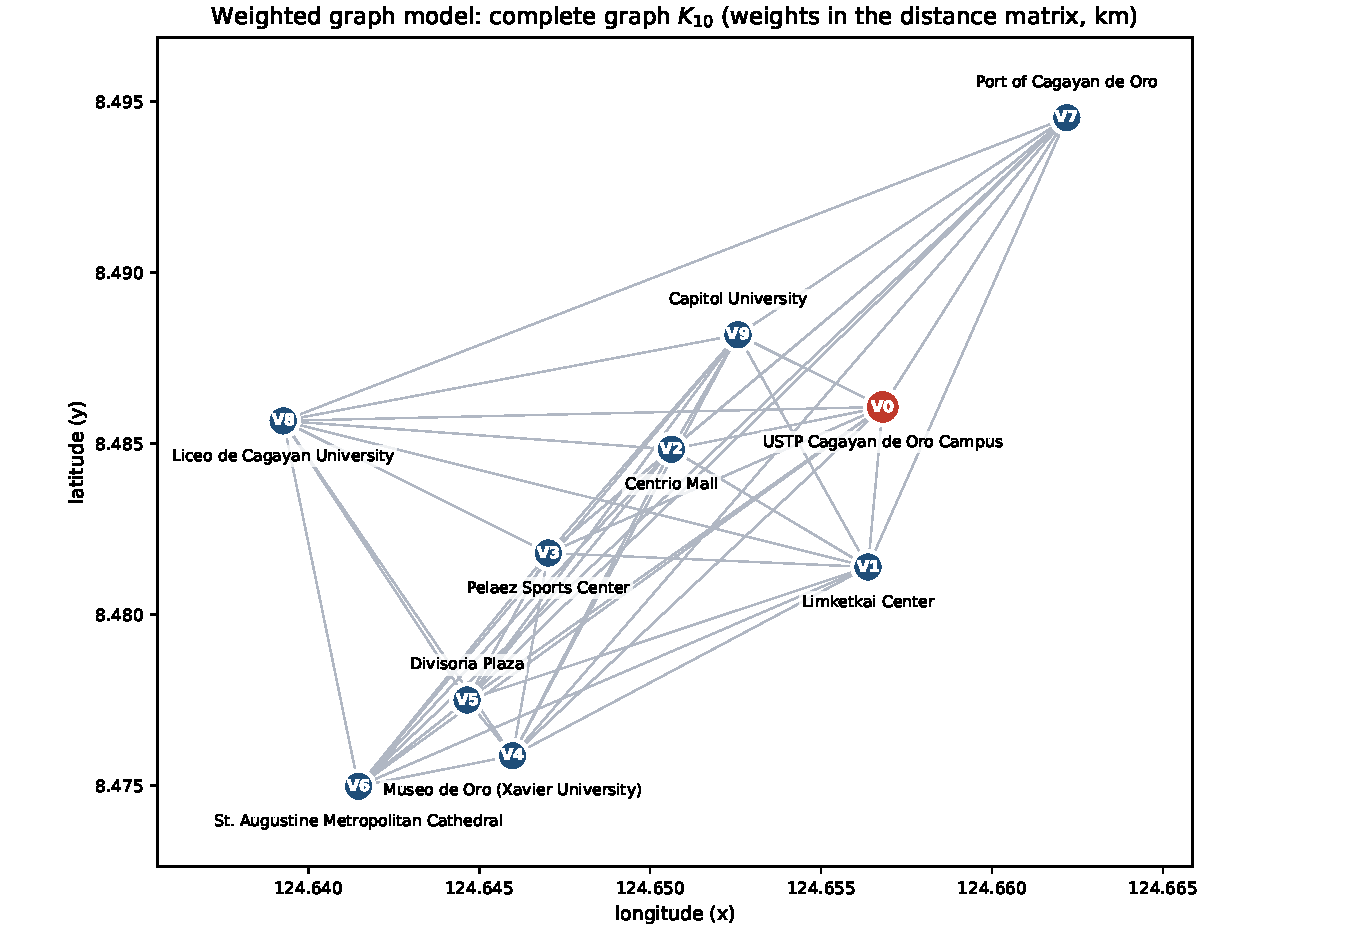
\includegraphics[width=0.85\textwidth]{graph.pdf}
\caption{Labelled graph model of downtown Cagayan de Oro. Every pair of locations is joined by an edge
(complete graph $K_{\NumVertices}$). Edge weights are listed in Table~\ref{tab:matrix}.}\label{fig:graph}
\end{figure}

\subsection{Edges and Weights}\label{sec:edges}
\paragraph{Edges.} An edge $\{u, v\}$ represents driving from location $u$ to location $v$ along the
shortest road route between them. Every location can be reached from every other, so $G$ is the
\textbf{complete graph} $K_{\NumVertices}$ with $\binom{\NumVertices}{2} = \NumEdges$ edges. An edge stands
for a whole road route, which may pass other locations without stopping; it is not a single street.

\paragraph{Direction.} We treat travel as \textbf{undirected}: $w(u,v) = w(v,u)$. The raw road distances are
slightly asymmetric because of one-way streets downtown (for example V0$\to$V1 is 1.00~km but V1$\to$V0 is
1.17~km in the raw data, \texttt{code/data/raw\_directed\_km.csv}). We set
\[
  w(u,v) = \tfrac12\bigl(d(u\to v) + d(v\to u)\bigr),
\]
rounded to 0.01~km. This keeps the model undirected, as the divide and conquer merge assumes.

\paragraph{Weights and units.} The weight $w(u,v)$ is the road distance in \textbf{kilometres (km)}.
Table~\ref{tab:matrix} is the complete weight matrix used by the program.

\begin{table}[H]
\centering
\caption{Edge weights $w(i,j)$: undirected road distance in km. The matrix is symmetric.}\label{tab:matrix}
\vspace{4pt}
\small
% AUTO-GENERATED by code/main.py --export-latex. Do not edit; re-run the export instead.
\begin{tabular}{l rrrrrrrrrr}
\toprule
 & \textbf{V0} & \textbf{V1} & \textbf{V2} & \textbf{V3} & \textbf{V4} & \textbf{V5} & \textbf{V6} & \textbf{V7} & \textbf{V8} & \textbf{V9} \\
\midrule
\textbf{V0} & -- & 1.09 & 1.26 & 1.94 & 2.48 & 2.37 & 2.83 & 2.07 & 2.62 & 1.34 \\
\textbf{V1} & 1.09 & -- & 1.55 & 2.24 & 2.10 & 2.21 & 2.50 & 2.32 & 2.96 & 1.68 \\
\textbf{V2} & 1.26 & 1.55 & -- & 1.18 & 1.55 & 1.61 & 1.85 & 2.17 & 1.86 & 0.58 \\
\textbf{V3} & 1.94 & 2.24 & 1.18 & -- & 1.31 & 0.97 & 1.43 & 2.98 & 2.15 & 1.38 \\
\textbf{V4} & 2.48 & 2.10 & 1.55 & 1.31 & -- & 0.54 & 0.87 & 3.52 & 1.92 & 1.93 \\
\textbf{V5} & 2.37 & 2.21 & 1.61 & 0.97 & 0.54 & -- & 0.74 & 3.29 & 1.58 & 1.70 \\
\textbf{V6} & 2.83 & 2.50 & 1.85 & 1.43 & 0.87 & 0.74 & -- & 3.87 & 1.65 & 2.28 \\
\textbf{V7} & 2.07 & 2.32 & 2.17 & 2.98 & 3.52 & 3.29 & 3.87 & -- & 3.66 & 1.79 \\
\textbf{V8} & 2.62 & 2.96 & 1.86 & 2.15 & 1.92 & 1.58 & 1.65 & 3.66 & -- & 2.06 \\
\textbf{V9} & 1.34 & 1.68 & 0.58 & 1.38 & 1.93 & 1.70 & 2.28 & 1.79 & 2.06 & -- \\
\bottomrule
\end{tabular}

\end{table}

\subsection{Data Sources: Actual and Assumed Data}\label{sec:data}

\begin{table}[H]
\centering
\caption{Sources of the data, separating actual data from assumptions.}\label{tab:sources}
\vspace{4pt}
\small
\begin{tabularx}{\textwidth}{l l >{\raggedright\arraybackslash}X}
\toprule
\textbf{Item} & \textbf{Type} & \textbf{Source / justification} \\
\midrule
Locations (V0--V9) & Actual & Real places in Cagayan de Oro City, located on Google
  Maps~\cite{googlemaps} and OpenStreetMap~\cite{osm}. \groupnote{Confirm each pin in Google Maps
  and add screenshots.} \\
Coordinates & Actual & OpenStreetMap, retrieved with the Nominatim geocoder~\cite{osm}. \\
Road distances $d(u\to v)$ & Actual & Shortest driving route on the OpenStreetMap road network,
  computed by the OSRM routing engine~\cite{luxen2011osrm} (\texttt{code/tools/build\_dataset.py}).
  \groupnote{Spot-check several pairs against Google Maps driving distances.} \\
Symmetric weights $w(u,v)$ & Assumed & Average of the two directions (Section~\ref{sec:edges}). \\
Travel mode, no traffic or time windows & Assumed & Simplifications listed in Section~\ref{sec:problem}. \\
Choice of the nine stops and the start & Assumed & Scenario chosen by the group. \\
\bottomrule
\end{tabularx}
\end{table}

All the data are in plain CSV files under \texttt{code/data/}:
\begin{itemize}
  \item \texttt{locations.csv}: the vertices (Table~\ref{tab:vertices});
  \item \texttt{distance\_matrix\_km.csv}: the edge weights (Table~\ref{tab:matrix});
  \item \texttt{raw\_directed\_km.csv}: the raw directed distances, before averaging.
\end{itemize}
The program reads these files directly, and every table
and figure in this report is generated from the same run of the program, so the graph, the data, the
program input and the reported results are consistent.

\subsection{Applying the Algorithm to the Graph}\label{sec:apply}
We run Algorithm~\ref{alg:dc} on $G$ with the paper's shortest-bridge merge (Algorithm~\ref{alg:merge})
and random seed \DCSeed{}. Fixing the seed makes the random choices, and so the result, reproducible.

\paragraph{Divide.} Figure~\ref{fig:tree} shows the recursion. Each box is a subset of vertices together
with the axis chosen to split it. The leaves are the base cases: one vertex (length 0), or two vertices
$a\to b\to a$ (length $2w(a,b)$).

\begin{figure}[H]
\centering
\resizebox{\textwidth}{!}{% AUTO-GENERATED by code/main.py --export-latex. Do not edit; re-run the export instead.
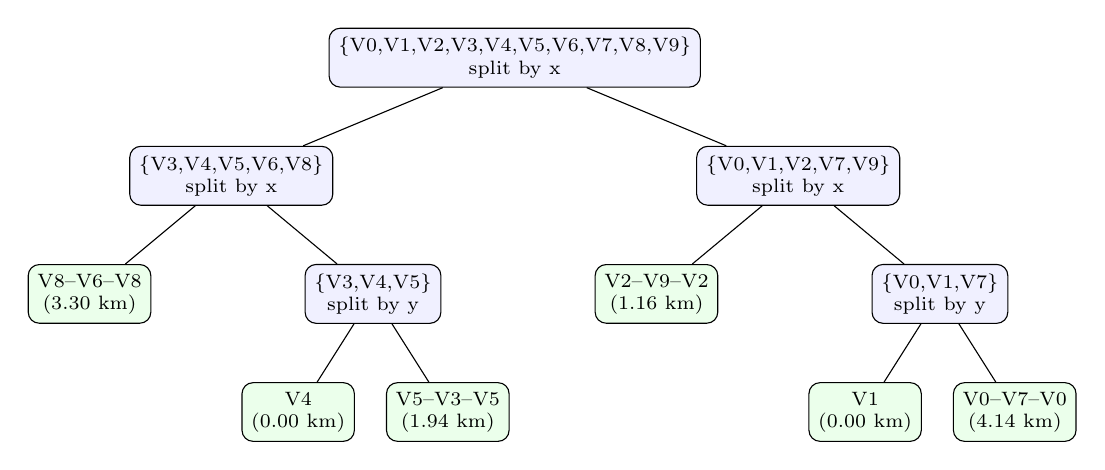
\begin{tikzpicture}[
  split/.style={draw, rounded corners, fill=blue!6, align=center, font=\scriptsize},
  leaf/.style={draw, rounded corners, fill=green!8, align=center, font=\scriptsize},
  level 1/.style={sibling distance=7.2cm, level distance=1.5cm},
  level 2/.style={sibling distance=3.6cm, level distance=1.5cm},
  level 3/.style={sibling distance=1.9cm, level distance=1.5cm}]
\node[split] {\{V0,V1,V2,V3,V4,V5,V6,V7,V8,V9\}\\split by x}
  child {
    node[split] {\{V3,V4,V5,V6,V8\}\\split by x}
    child {
      node[leaf] {V8--\allowbreak V6--\allowbreak V8\\(3.30 km)}
    }
    child {
      node[split] {\{V3,V4,V5\}\\split by y}
      child {
        node[leaf] {V4\\(0.00 km)}
      }
      child {
        node[leaf] {V5--\allowbreak V3--\allowbreak V5\\(1.94 km)}
      }
    }
  }
  child {
    node[split] {\{V0,V1,V2,V7,V9\}\\split by x}
    child {
      node[leaf] {V2--\allowbreak V9--\allowbreak V2\\(1.16 km)}
    }
    child {
      node[split] {\{V0,V1,V7\}\\split by y}
      child {
        node[leaf] {V1\\(0.00 km)}
      }
      child {
        node[leaf] {V0--\allowbreak V7--\allowbreak V0\\(4.14 km)}
      }
    }
  };
\end{tikzpicture}
}
\caption{Divide step for seed \DCSeed{}: recursive median splits by longitude ($x$) or latitude ($y$).
Leaves show the base-case tours and their lengths in km.}\label{fig:tree}
\end{figure}

\paragraph{The same run on the map.} Figure~\ref{fig:steps} draws the recursion on the graph itself.
Panel~(a) shows the median cuts, numbered by recursion level: the level-1 cut is the vertical line that
splits the ten vertices into a western and an eastern half, and the level-2 and level-3 cuts split those
halves again. Panel~(b) shows the base cases: pairs joined by an edge, and single vertices (V1, V4).
Panel~(c)--(e) then undo the cuts from the deepest level up. At each level the sub-tours on the two
sides of a cut are merged by deleting one edge from each (dashed red) and adding the shortest bridge
and a closing edge (gold). After the level-1 merge a single Hamiltonian cycle remains, which is the
final tour. The edge $V_8$--$V_0$ passes visually near $V_2$ in the map, but it is one direct graph
edge; passing near another marker does not visit that vertex or add an extra stop.

\begin{figure}[H]
\centering
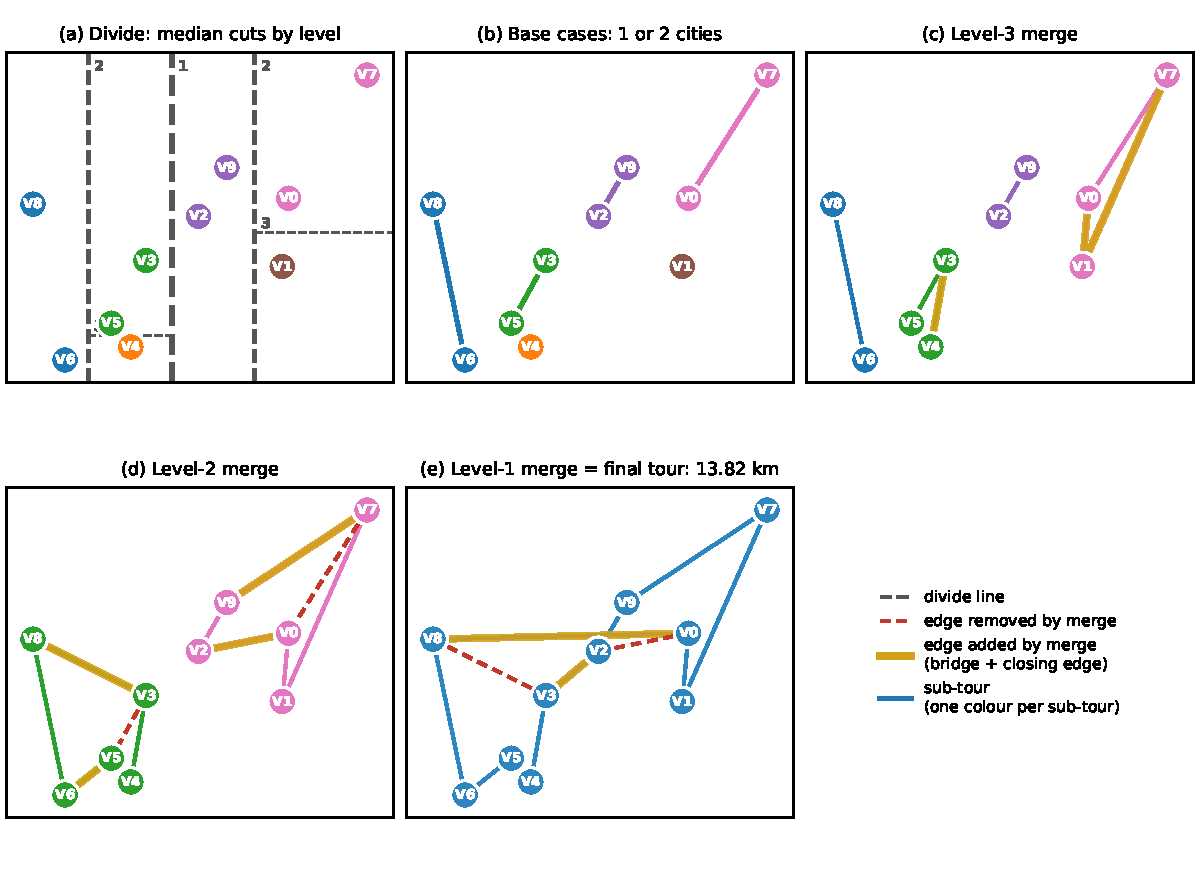
\includegraphics[width=\textwidth]{steps.pdf}
\caption{Divide and Conquer on the graph (seed \DCSeed{}). (a)~Divide lines; (b)~base-case
sub-tours, one colour per sub-tour; (c)--(e)~merges from the deepest level to the top. Dashed red
edges are removed and gold edges are added by a merge. When a two-city tour $a\to b\to a$ is merged,
only one copy of its doubled edge is removed, so that edge stays visible.}\label{fig:steps}
\end{figure}

\paragraph{Conquer and combine.} The sub-tours are merged bottom-up. Table~\ref{tab:trace} lists every
merge: the two input cycles, the shortest bridge, the edges removed and added, the change in length
$\Delta$, and the length of the merged cycle. Each row satisfies
$L(T) = L(T_1) + L(T_2) + \Delta$.

\begin{table}[H]
\centering
\caption{Merge steps (bottom-up). Edge weights in km are given in parentheses.}\label{tab:trace}
\vspace{4pt}
\scriptsize
\setlength{\tabcolsep}{3pt}
% AUTO-GENERATED by code/main.py --export-latex. Do not edit; re-run the export instead.
\begin{tabular}{c >{\raggedright\arraybackslash}p{2.6cm} >{\raggedright\arraybackslash}p{2.6cm} >{\raggedright\arraybackslash}p{1.9cm} >{\raggedright\arraybackslash}p{2.45cm} >{\raggedright\arraybackslash}p{2.45cm} r r}
\toprule
\textbf{Step} & \textbf{Left tour (km)} & \textbf{Right tour (km)} & \textbf{Shortest bridge} & \textbf{Edges removed} & \textbf{Edges added} & $\boldsymbol{\Delta}$ & \textbf{Merged} \\
\midrule
M1 & V4 (0.00) & V5--\allowbreak V3--\allowbreak V5 (1.94) & V4--V5 (0.54) & V5--V3 (0.97) & V4--V3 (1.31), V5--V4 (0.54) & +0.88 & 2.82 \\
M2 & V8--\allowbreak V6--\allowbreak V8 (3.30) & V4--\allowbreak V3--\allowbreak V5--\allowbreak V4 (2.82) & V6--V5 (0.74) & V8--V6 (1.65), V3--V5 (0.97) & V8--V3 (2.15), V5--V6 (0.74) & +0.27 & 6.39 \\
M3 & V1 (0.00) & V0--\allowbreak V7--\allowbreak V0 (4.14) & V1--V0 (1.09) & V0--V7 (2.07) & V1--V7 (2.32), V0--V1 (1.09) & +1.34 & 5.48 \\
M4 & V2--\allowbreak V9--\allowbreak V2 (1.16) & V1--\allowbreak V7--\allowbreak V0--\allowbreak V1 (5.48) & V2--V0 (1.26) & V2--V9 (0.58), V7--V0 (2.07) & V2--V0 (1.26), V7--V9 (1.79) & +0.40 & 7.04 \\
M5 & V6--\allowbreak V8--\allowbreak V3--\allowbreak V4--\allowbreak V5--\allowbreak V6 (6.39) & V9--\allowbreak V2--\allowbreak V0--\allowbreak V1--\allowbreak V7--\allowbreak V9 (7.04) & V3--V2 (1.18) & V8--V3 (2.15), V2--V0 (1.26) & V8--V0 (2.62), V2--V3 (1.18) & +0.39 & 13.82 \\
\bottomrule
\end{tabular}

\end{table}

\paragraph{Worked calculation of the final merge.}
% AUTO-GENERATED by code/main.py --export-latex. Do not edit; re-run the export instead.
The two halves return the sub-tours $T_1 = $ V6--\allowbreak V8--\allowbreak V3--\allowbreak V4--\allowbreak V5--\allowbreak V6 (length 6.39 km) and $T_2 = $ V9--\allowbreak V2--\allowbreak V0--\allowbreak V1--\allowbreak V7--\allowbreak V9 (length 7.04 km).
Checking all $|T_1|\cdot|T_2| = 5\cdot5 = 25$ cross pairs, the shortest bridge is V3--V2 with $w = 1.18$ km.
Among the ways of opening one edge next to each bridge endpoint and closing the loop, the cheapest removes V8--V3 and V2--V0 and adds V8--V0 and V2--V3:
\[\Delta = (2.62 + 1.18) - (2.15 + 1.26) = +0.39\text{ km},\]
\[L(T) = L(T_1) + L(T_2) + \Delta = 6.39 + 7.04 + 0.39 = 13.82\text{ km}.\]
The merged cycle is V3--\allowbreak V4--\allowbreak V5--\allowbreak V6--\allowbreak V8--\allowbreak V0--\allowbreak V1--\allowbreak V7--\allowbreak V9--\allowbreak V2--\allowbreak V3, which visits all 10 vertices once.


Finally, the cycle is rotated to begin at V0, giving the closed route
\begin{center}
\DCRoute{}
\end{center}
of length \textbf{\DCTotal{} km}.


\section{Python Implementation}\label{sec:implementation}

\subsection{Main Code Components}
The program is written in Python~3 using only the standard library; matplotlib~\cite{hunter2007matplotlib}
is used for the figures. Table~\ref{tab:components} maps each part of the algorithm to the code, and the
full source of the algorithm is in Appendix~\ref{app:code}.

\begin{table}[H]
\centering
\caption{Main code components (folder \texttt{code/}).}\label{tab:components}
\vspace{4pt}
\small
\begin{tabularx}{\textwidth}{l l >{\raggedright\arraybackslash}X}
\toprule
\textbf{File} & \textbf{Function} & \textbf{Role in the algorithm} \\
\midrule
\texttt{data/*.csv} & -- & Input data: vertices (\texttt{locations.csv}) and weights (\texttt{distance\_matrix\_km.csv}). \\
\texttt{main.py} & \texttt{load\_locations}, \texttt{load\_matrix} & Read the data and check that the matrix is square, symmetric and has a zero diagonal. \\
\texttt{dc\_tsp.py} & \texttt{divide\_and\_conquer\_tsp} & Entry point: shuffle (Step 1), recurse, rotate the final cycle to start at V0. \\
 & \texttt{split} & Divide (Step 2): random axis, sort, cut at the median. \\
 & \texttt{solve} & Recursion: base cases (Step 3), conquer both halves (Step 4), merge; records a trace of every step. \\
 & \texttt{shortest\_bridge} & Closest cross pair $(a,b)$, $O(n^2)$ (Step 5). \\
 & \texttt{merge} & Remove one edge per cycle, add the bridge and a closing edge, keep the smallest $\Delta$ (Steps 5--6, Algorithm~\ref{alg:merge}). \\
\texttt{verify.py} & \texttt{check\_route} & Checks the route is a valid closed tour and recomputes its length from the weights. \\
 & \texttt{held\_karp} & Exact optimum for comparison only (not part of the assigned algorithm). \\
\texttt{test\_dc\_tsp.py} & -- & Automated tests: valid tours on random instances of 1--39 cities; Held--Karp agrees with brute force. \\
\texttt{plots.py}, \texttt{export\_latex.py} & -- & Figures, and the tables used in this report. \\
\bottomrule
\end{tabularx}
\end{table}

The coordinates are used \emph{only} in \texttt{split}. Every length (bridges, $\Delta$, the total) is
computed from the road-distance matrix, so the result is measured in road kilometres, not straight-line
distance.

\subsection{Running the Program}
From the \texttt{code/} folder:
\begin{lstlisting}[language=bash, numbers=none]
python main.py                 # seed 1, shortest-bridge merge (results in this report)
python main.py --seed 7        # another random run
python main.py --rule best     # alternative best-splice merge
python main.py --export-latex  # also regenerate the report's tables and figures
\end{lstlisting}

The program prints, in order: (1) the input data, meaning the vertex table and the weight matrix;
(2) every divide, base-case and merge step, with the arithmetic of each merge; (3) the resulting route as
a table of legs with cumulative distance; (4) the verification checks; (5) the comparison with the exact
optimum; and (6) statistics over \RunCount{} seeds. The same output is shown in the screen recording of
our presentation. \groupnote{Add a screenshot of the terminal output here if required.}

\subsection{Verification of the Output}\label{sec:verification}
The function \texttt{check\_route} confirms that the route (i) starts at V0, (ii) ends at V0, (iii) has
$\NumVertices + 1$ entries, i.e.\ \NumVertices{} legs, and (iv) contains every vertex V0--V9 exactly once
before returning to V0. It then \textbf{recomputes the total independently} by adding the matrix weight of
each leg (Table~\ref{tab:legs}). For our run all checks \DCAllChecks{}, and the recomputed total is
\DCRecomputed{}~km, equal to the \DCTotal{}~km reported by the algorithm.

In addition, \texttt{test\_dc\_tsp.py} runs both merge rules on random instances with 1 to 39 cities and
5 seeds each, and checks that every output is a valid closed tour whose recomputed length matches. It
also checks that the Held--Karp baseline agrees with brute force for 3 to 8 cities, and that the
heuristic is never shorter than the optimum.


\section{Solution and Conclusion}\label{sec:conclusion}

\subsection{Resulting Route}\label{sec:results}
With seed \DCSeed{}, the Divide and Conquer algorithm returns the closed route
\begin{center}
\DCRoute{}
\end{center}
with a total driving distance of \textbf{\DCTotal{} km}. Table~\ref{tab:legs} gives each leg, and
Figure~\ref{fig:route} draws the route on the map.

\begin{table}[H]
\centering
\caption{Legs of the Divide and Conquer route and the recomputed total (km).}\label{tab:legs}
\vspace{4pt}
\footnotesize
\setlength{\tabcolsep}{3.5pt}
% AUTO-GENERATED by code/main.py --export-latex. Do not edit; re-run the export instead.
\begin{tabular}{c l l r r}
\toprule
\textbf{Leg} & \textbf{From} & \textbf{To} & \textbf{km} & \textbf{Cumulative} \\
\midrule
1 & V0 USTP Cagayan de Oro Campus & V1 Limketkai Center & 1.09 & 1.09 \\
2 & V1 Limketkai Center & V7 Port of Cagayan de Oro & 2.32 & 3.41 \\
3 & V7 Port of Cagayan de Oro & V9 Capitol University & 1.79 & 5.20 \\
4 & V9 Capitol University & V2 Centrio Mall & 0.58 & 5.78 \\
5 & V2 Centrio Mall & V3 Pelaez Sports Center & 1.18 & 6.96 \\
6 & V3 Pelaez Sports Center & V4 Museo de Oro (Xavier University) & 1.31 & 8.27 \\
7 & V4 Museo de Oro (Xavier University) & V5 Divisoria Plaza & 0.54 & 8.81 \\
8 & V5 Divisoria Plaza & V6 St. Augustine Metropolitan Cathedral & 0.74 & 9.55 \\
9 & V6 St. Augustine Metropolitan Cathedral & V8 Liceo de Cagayan University & 1.65 & 11.20 \\
10 & V8 Liceo de Cagayan University & V0 USTP Cagayan de Oro Campus & 2.62 & 13.82 \\
\midrule
\multicolumn{3}{r}{\textbf{Total}} & \multicolumn{2}{r}{\textbf{13.82 km}} \\
\bottomrule
\end{tabular}

\end{table}

\begin{figure}[H]
\centering
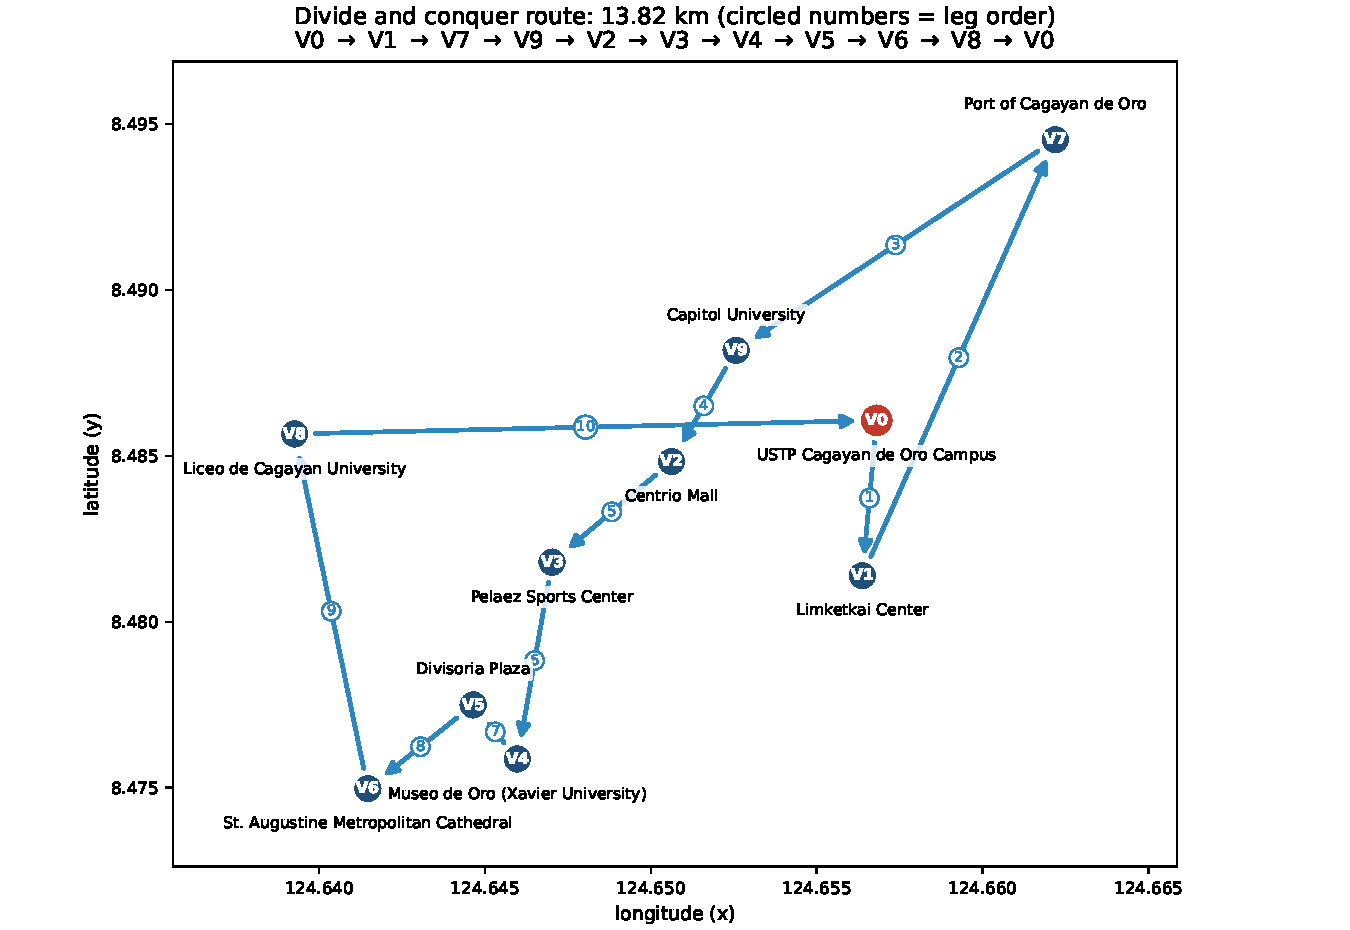
\includegraphics[width=0.85\textwidth]{route.pdf}
\caption{Divide and Conquer route (seed \DCSeed{}). Circled numbers give the order of the legs.}\label{fig:route}
\end{figure}

\paragraph{Interpretation.} The route meets the objective's constraints: the guests leave USTP, visit
each of the nine landmarks exactly once, and return to USTP. It forms one loop: south to Limketkai,
north to the port, then south-west through Capitol University, Centrio, Pelaez, Museo de Oro,
Divisoria and the Cathedral, and finally north-west to Liceo before heading back east to USTP. Because the divide step groups
nearby places, the tight cluster around Divisoria (V4, V5, V6) is visited consecutively using its
shortest edges (0.54 and 0.74~km). The weakest part is the last leg, Liceo (V8) back to USTP
(2.62~km). It was created by the final merge (Table~\ref{tab:trace}), which had to reconnect the two
halves through the shortest bridge V2--V3 and therefore closed the loop with the long edge V8--V0.
This is the ``boundary effect'' limitation of Section~\ref{sec:algorithm} appearing in practice.

\subsection{Is the Route Optimal?}\label{sec:optimality}
Divide and Conquer gives no proof of optimality, so we checked the result separately. With only
\NumVertices{} vertices, the exact Held--Karp algorithm~\cite{heldkarp1962} (Algorithm~2.2 of the
paper) can be run in well under a second. It gives the provably optimal tour
\begin{center}
\OptRoute{}
\end{center}
of length \textbf{\OptTotal{} km}. Our Divide and Conquer route is therefore \textbf{not optimal}: it is
\DCTotal{} km, i.e.\ \DCGap\% longer than the optimum. It is an \emph{approximate} solution.

Because the algorithm is randomised, we also repeated it with \RunCount{} different seeds, as the paper does
in its Table~2. Table~\ref{tab:experiments} summarises the results.

\begin{table}[H]
\centering
\caption{Tour length (km) over \RunCount{} seeds, compared with the exact optimum. ``Optimal'' counts the runs
that reached the optimum.}\label{tab:experiments}
\vspace{4pt}
\small
% AUTO-GENERATED by code/main.py --export-latex. Do not edit; re-run the export instead.
\begin{tabular}{l r r r r r r r}
\toprule
\textbf{Method} & \textbf{Best} & \textbf{Worst} & \textbf{Mean} & \textbf{Std.} & \textbf{Mean gap} & \textbf{Optimal} & \textbf{ms/run} \\
\midrule
Shortest bridge (paper) & 13.61 & 14.26 & 13.88 & 0.25 & 2.01\% & 6/100 & 0.405 \\
Best splice (variant) & 13.61 & 14.13 & 13.91 & 0.24 & 2.20\% & 17/100 & 0.342 \\
Held--Karp (exact) & 13.61 & 13.61 & 13.61 & 0.00 & 0.00\% & -- & -- \\
\bottomrule
\end{tabular}

\end{table}

With the paper's shortest-bridge merge, the tour length ranged from \BridgeBest{} to \BridgeWorst{}~km
(mean \BridgeMean{}~km, \BridgeMeanGap\% above optimal). Only \BridgeOptHits{} of the \RunCount{} runs
happened to produce an optimal tour, and the algorithm itself cannot recognise when this happens; only
the separate Held--Karp check shows it. This confirms that the method is a heuristic: on its own it
gives a good tour, not a proven optimal one.

\subsection{Limitations and Possible Improvements}\label{sec:limitations}
\paragraph{Limitations of the solution.}
\begin{itemize}
      \item The route is approximate (1.54\% above optimal), and it depends on the
            random seed: the 100-seed results in Table~\ref{tab:experiments} range from
            13.61 to 14.26 km.
  \item Distance is the only cost. Traffic, travel time, opening hours and the time spent at each stop
        are ignored, although they matter for a real one-day tour.
  \item Weights are made symmetric by averaging, so one-way streets are only approximated (this route is
        13.54 km on the raw one-way values).
  \item Road distances come from OpenStreetMap routing. A Google Maps check of
        the final route gave 14.40 km against 13.82 km (+4.2\%), with individual
        legs differing by up to 39\% (Table~\ref{tab:gmaps}). The optimality
        statement of Section~5.2 holds for the OSRM matrix only; we did not
        recompute the optimum with Google distances.
\end{itemize}

\paragraph{Improvements.}
\begin{itemize}
  \item \textbf{Local search after merging.} Applying 2-opt or Or-opt moves to
        the final tour removes locally poor orderings and usually closes most of
        the remaining gap~\cite{applegate2006tsp}. On our route, a single 2-opt
        move that reverses the segment $V_4 \to V_5$ replaces the edges
        $V_3$--$V_4$ (1.31 km) and $V_5$--$V_6$ (0.74 km) by $V_3$--$V_5$
        (0.97 km) and $V_4$--$V_6$ (0.87 km). This saves $2.05 - 1.84 = 0.21$
        km and gives exactly the optimal length of 13.61 km.
  \item \textbf{Multiple restarts.} Run several seeds and keep the shortest tour. Each run takes about
        0.3~ms here, and the best of \RunCount{} runs was \BridgeBest{}~km. This equals the optimum
        only because the separate Held--Karp computation identifies it; restarts alone do not prove
        optimality.
  \item \textbf{Merge rule.} We also tested the best-splice rule, which may
        break any edge of either sub-tour rather than only the edges next to the
        shortest bridge. On this instance it reached the optimum more often (17 vs.\
        6 runs), but its mean length was 13.91 km against 13.88 km
        (Table~\ref{tab:experiments}). A cheaper merge at each step does not
        guarantee a shorter final tour, because every merge is still a local,
        irreversible decision.
  \item \textbf{Richer weights.} Use travel time with traffic from Google Maps, or a directed (asymmetric)
        matrix, if the objective changes from distance to time.
  \item \textbf{Exact methods for small instances.} For about 15 stops or fewer, Held--Karp is fast
        enough to give the true optimum. Divide and Conquer is most useful when $n$ is too large for that.
\end{itemize}

\subsection{Conclusion}
We modelled a one-day city tour of downtown Cagayan de Oro as a TSP on the complete undirected graph
$K_{\NumVertices}$, with road distances in kilometres as weights, and solved it with the Divide and
Conquer algorithm of Luna-Garcia et al.~\cite{lunagarcia2024performance}. The paper's merge code does
not produce a valid tour, so we implemented the merge as a proper cycle splice through the shortest
bridge, which keeps the algorithm's $O(n^2)$ running time. The program found the closed route
\DCRoute{} of \DCTotal{}~km; we verified that it visits every location exactly once and recomputed
its length from the weights. Compared with the exact optimum of \OptTotal{}~km, the route is
\DCGap\% longer. Divide and Conquer therefore gave a fast, valid, \emph{approximate} tour, not a
proven optimal one; a local-search pass or several restarts would improve it.



\bibliographystyle{plain}
\bibliography{dc-tsp-refs}

\begin{appendices}
\section{Source Code}\label{app:code}
The complete program and dataset are submitted in the folder \texttt{code/}. The input data are in
\texttt{code/data/locations.csv} and \texttt{code/data/distance\_matrix\_km.csv}.

\subsection{Algorithm: \texttt{dc\_tsp.py}}
\lstinputlisting{../../code/dc_tsp.py}

\subsection{Verification: \texttt{verify.py}}
\lstinputlisting{../../code/verify.py}

\end{appendices}
\end{document}
